\documentclass[bachelor]{njupthesis}

\title{这是标题}
\author{这是你的名字}
\advisor{导师的名字}
\school{南京邮电大学某某学院}
\major{某某专业}
\studentclass{Q/B17xxxx} % 班级号,可以不填,留空则不显示
\studentid{Q/B21xxxxxx} % 学号
\graduateyear{2025} % 毕业年份(页眉)
\begindate{202x年x月x日} % 封面毕设开始时间
\finishdate{202x年x月x日} % 封面毕设结束时间
\createdate{2025}{5}{30} % 毕设原创性声明日期,不需要可以三个全留空,但不可以删除花括号

% 作者签名和导师电子签名,电子签名图片需要放入pic目录下,留空则不添加签名
% 注意,签名图片上下不要留过多空白,最好只包含电子签名的文字本身,否则会影响嵌入效果
\authorsign{示例签名} % 作者签名在原创性声明中显示,留空不添加任何内容
\advisorsign{} % 导师签名在封面显示,留空则以普通文字显示导师名字

\begin{document} % 论文内容开始,禁止删除

\makecover % 生成封面、原创性声明,禁止删除

\begin{chineseabstract} % 中文摘要
南京南站(Nanjingnan Railway Station)位于江苏省南京市雨花台区,是中国铁路上海局集团有限公司管辖的客运站,是南京铁路枢纽的重要组成部分,也是华东地区最大的交通枢纽 ,国家铁道枢纽站 ,是亚洲第一大火车站。
南京南站规划于1986年,地处南京南部新城的核心区;1991年进入早期规划阶段;2008年1月正式开工,北靠雨花台风景区、南临秦淮新河、西接牛首山;2008年8月规划设计方案最终确定;2011年6月28日南京南站及北广场正式投入使用,成为中国第一个通过垂直换乘实现真正零换乘的交通枢纽,其“垂直换乘”的设计理念被铁道部全面推广和使用。 
截至2019年12月,南京南站占地面积约70万平方米,总建筑面积73万平方米,站房总建筑面积约45.8万平方米,其中主站房面积达38.7万平方米,是亚洲最大的火车站,总投资超过300亿元人民币,站房建筑秉承“古都新站”的设计理念,吸纳了大量中国古典建筑元素,如藻井、斗拱、窗花和木纹肌理等,同时中西合璧、兼收并蓄,将中国宫殿建筑的优势及特点充分发挥,体现了古都南京浓郁的风格和特有的气质。


\chinesekeyword{南京南站;铁道部;京沪高铁;南京} % 中文关键词
\end{chineseabstract}

\begin{englishabstract} % 英文摘要
Nanjingnan Railway Station is located in Yuhuatai District, Nanjing city, Jiangsu Province. It is a passenger Station under the jurisdiction of China Railway Shanghai Group Co., LTD. It is an important part of Nanjing Railway Hub, the largest transportation hub in East China, the national Railway hub Station, and the largest Railway Station in Asia.
Planned in 1986, Nanjing South Railway Station is located in the core area of the new city in the south of Nanjing. It entered the early planning stage in 1991; Construction started in January 2008, with Yuhuatai Scenic Spot in the north, Qinhuai New River in the south and Niushou Mountain in the west. In August 2008, the planning and design scheme was finalized; On June 28, 2011, Nanjing South Railway Station and North Plaza were officially put into use, becoming the first transportation hub in China to realize real zero transfer through vertical transfer. Its design concept of "vertical transfer" was fully promoted and used by the Ministry of Railways.
As of December 2019, the nanjing south railway station area of about 700000 square meters, a total construction area of 730000 square meters, the station building a total construction area of 458000 square meters, of which the main room area of 387000 square meters, is Asia's largest railway station, with a total investment of more than 30 billion yuan, the station building adhering to the "ancient capital of xinzhan" design concept, Absorbing a large number of Chinese classical architectural elements, such as sunk panels, brackets, window cuts and wood texture, etc., the combination of Chinese and Western elements, eclectic, gives full play to the advantages and characteristics of Chinese palace architecture, reflecting the rich style and unique temperament of the ancient capital Nanjing.

\englishkeyword{Nanjing South Railway Station; Railway; Nanjing} % 英文关键词
\end{englishabstract}

\thesistableofcontents % 生成目录,禁止删除

\thesischapterexordium % 正文开始,禁止删除

\chapter{绪论}
1986年,南京市整体规划向南发展,决定在主城南部建设大型车站,并预留了南京南站地区的规划空间。
1990年12月,原中华人民共和国铁道部完成《京沪高速铁路线路方案构想报告》。京沪高铁的前期工作进展,极为缓慢,甚至搁浅停滞相当长的一段时间,铁路要在速度上与民航竞争很多人持怀疑态度。
1991年,南京南站进入早期规划阶段。

\section{名字自己替换(二级标题)}
\subsection{名字自己替换(三级标题)}
1994年12月,中国国务院批准开展京沪高速铁路预可行性研究。铁道部开展京沪高铁选线,提出“北线方案”,即从上元门地区,通过隧道过江。南京的规划部门则拿出“南线方案”,从大胜关过江。铁道部牵头,进行比选得出的结论是:两个方案在技术上都可行,主要差别在于工程造价、经济效益、运营条件等方面。江苏省和南京市要求南线方案,而铁道部看好的始终是北线方案。南京力主南线,是放长了眼光。如果从南京北部走,已经不具备扩建条件。南京火车站虽然前面是玄武湖、背面是小红山,景观很美,但是已经没有拓展空间。此外,更重要的是,在全国任何一个城市,铁路带动城市发展的效果都非常明显,南京要想进一步发展南部区域,这是个好机会。显然,高铁建在哪里,也就意味着南京今后的发展框架,是继续囿于老城狭小的空间里,还是大步向南拓展。铁道部青睐北线的理由:新线与既有线的衔接方便。清末修建的津浦铁路,即从天津到浦口;在长江南岸,之后又修建了沪宁铁路。浦口火车站、下关火车站、南京站,南京重要的火车站,向来都是位于城北。并且,当时铁道部的人都认为,南京的城市中心就在北边。另一方面,铁路的机务段、职工宿舍等都在城北,建成之后,职工上下班都方便。为了说服铁道部,南京方面列出了南线的九大优势:无论高铁从哪里走,从完善南京枢纽总体布局的角度来看,都必须建大胜关长江大桥;根据国务院批准的南京城市规划,南京城市今后将主要向东南方向发展,大胜关方案符合城市扩展方向;南面的场站位置已预留多年,有较为理想的建站条件;沿线拆迁量小,对城市干扰和环境影响小;利于形成方便的铁路——航空换乘及铁路与城市道路联结条件……不过,这些最初并没有打动铁道部,铁道部仍然坚持北线方,双方为此对峙了好几年。


\subsection{名字自己替换}
1995年,为了促进高铁尽快上马,南京稍稍“松口”。在当年的一份紧急报告里,有这样一句话——“南北方案之争不宜过多坚持,而从规划上对北线方案提出完善意见为妥”。南京市规划局做了两手准备,针对南线、北线方案,分别做了规划控制。从1995年起,南京根据两个方案,开始分别严格控制沿线用地建设,同时冻结了南北两条线周围的土地。而这个具有预见性的做法,使得后来的工作变得轻松许多。

\section{俄罗斯和乌克兰}
本论文主要创新点与贡献如下\cite{荣洁2005俄罗斯民族性格和文化}:

xxxxxxxxxxxxxx


\section{什么是快乐星球}
本文的章节结构安排如下:

xxxxxxx


\chapter{第二章了!}

第二章主要给大家演示一下各种LaTex的编写格式,首先要注意的是,LaTex中空行是不会被渲染出来的,main.tex中行与行之间留一个空行就代表分段。

\section{格式演示}

\subsection{这是三级标题}

最多就是三级标题了,超过三级标题请使用(1)和1.的格式来编写小标题。

(1)参考文献

这是一个参考文献示例\cite{PRODEN},cite之后会自动更新最后的参考文献列表。同时参考文献也会自动编号、双向引用。在同一篇论文中可以多次cite同一篇参考文献,比如这样\cite{PRODEN},序号会保持相同。

请注意,如果引用的论文是EB/OL或者包含了url链接,则需要在bib里面提供urldate作为引用日期或者更新日期,否则不符合学校要求的参考文献引用格式。

(2)单图片

下面给出单个图片的格式,其中"{texpage截图}"是这个图片的名字,需要将图片源文件放入pic目录下;width是一个百分比,控制图片大小;caption就是图注内容;label是图片的latex编号,通过图\ref{fig:2}来引用这张图片。
\begin{figure}[htbp]
    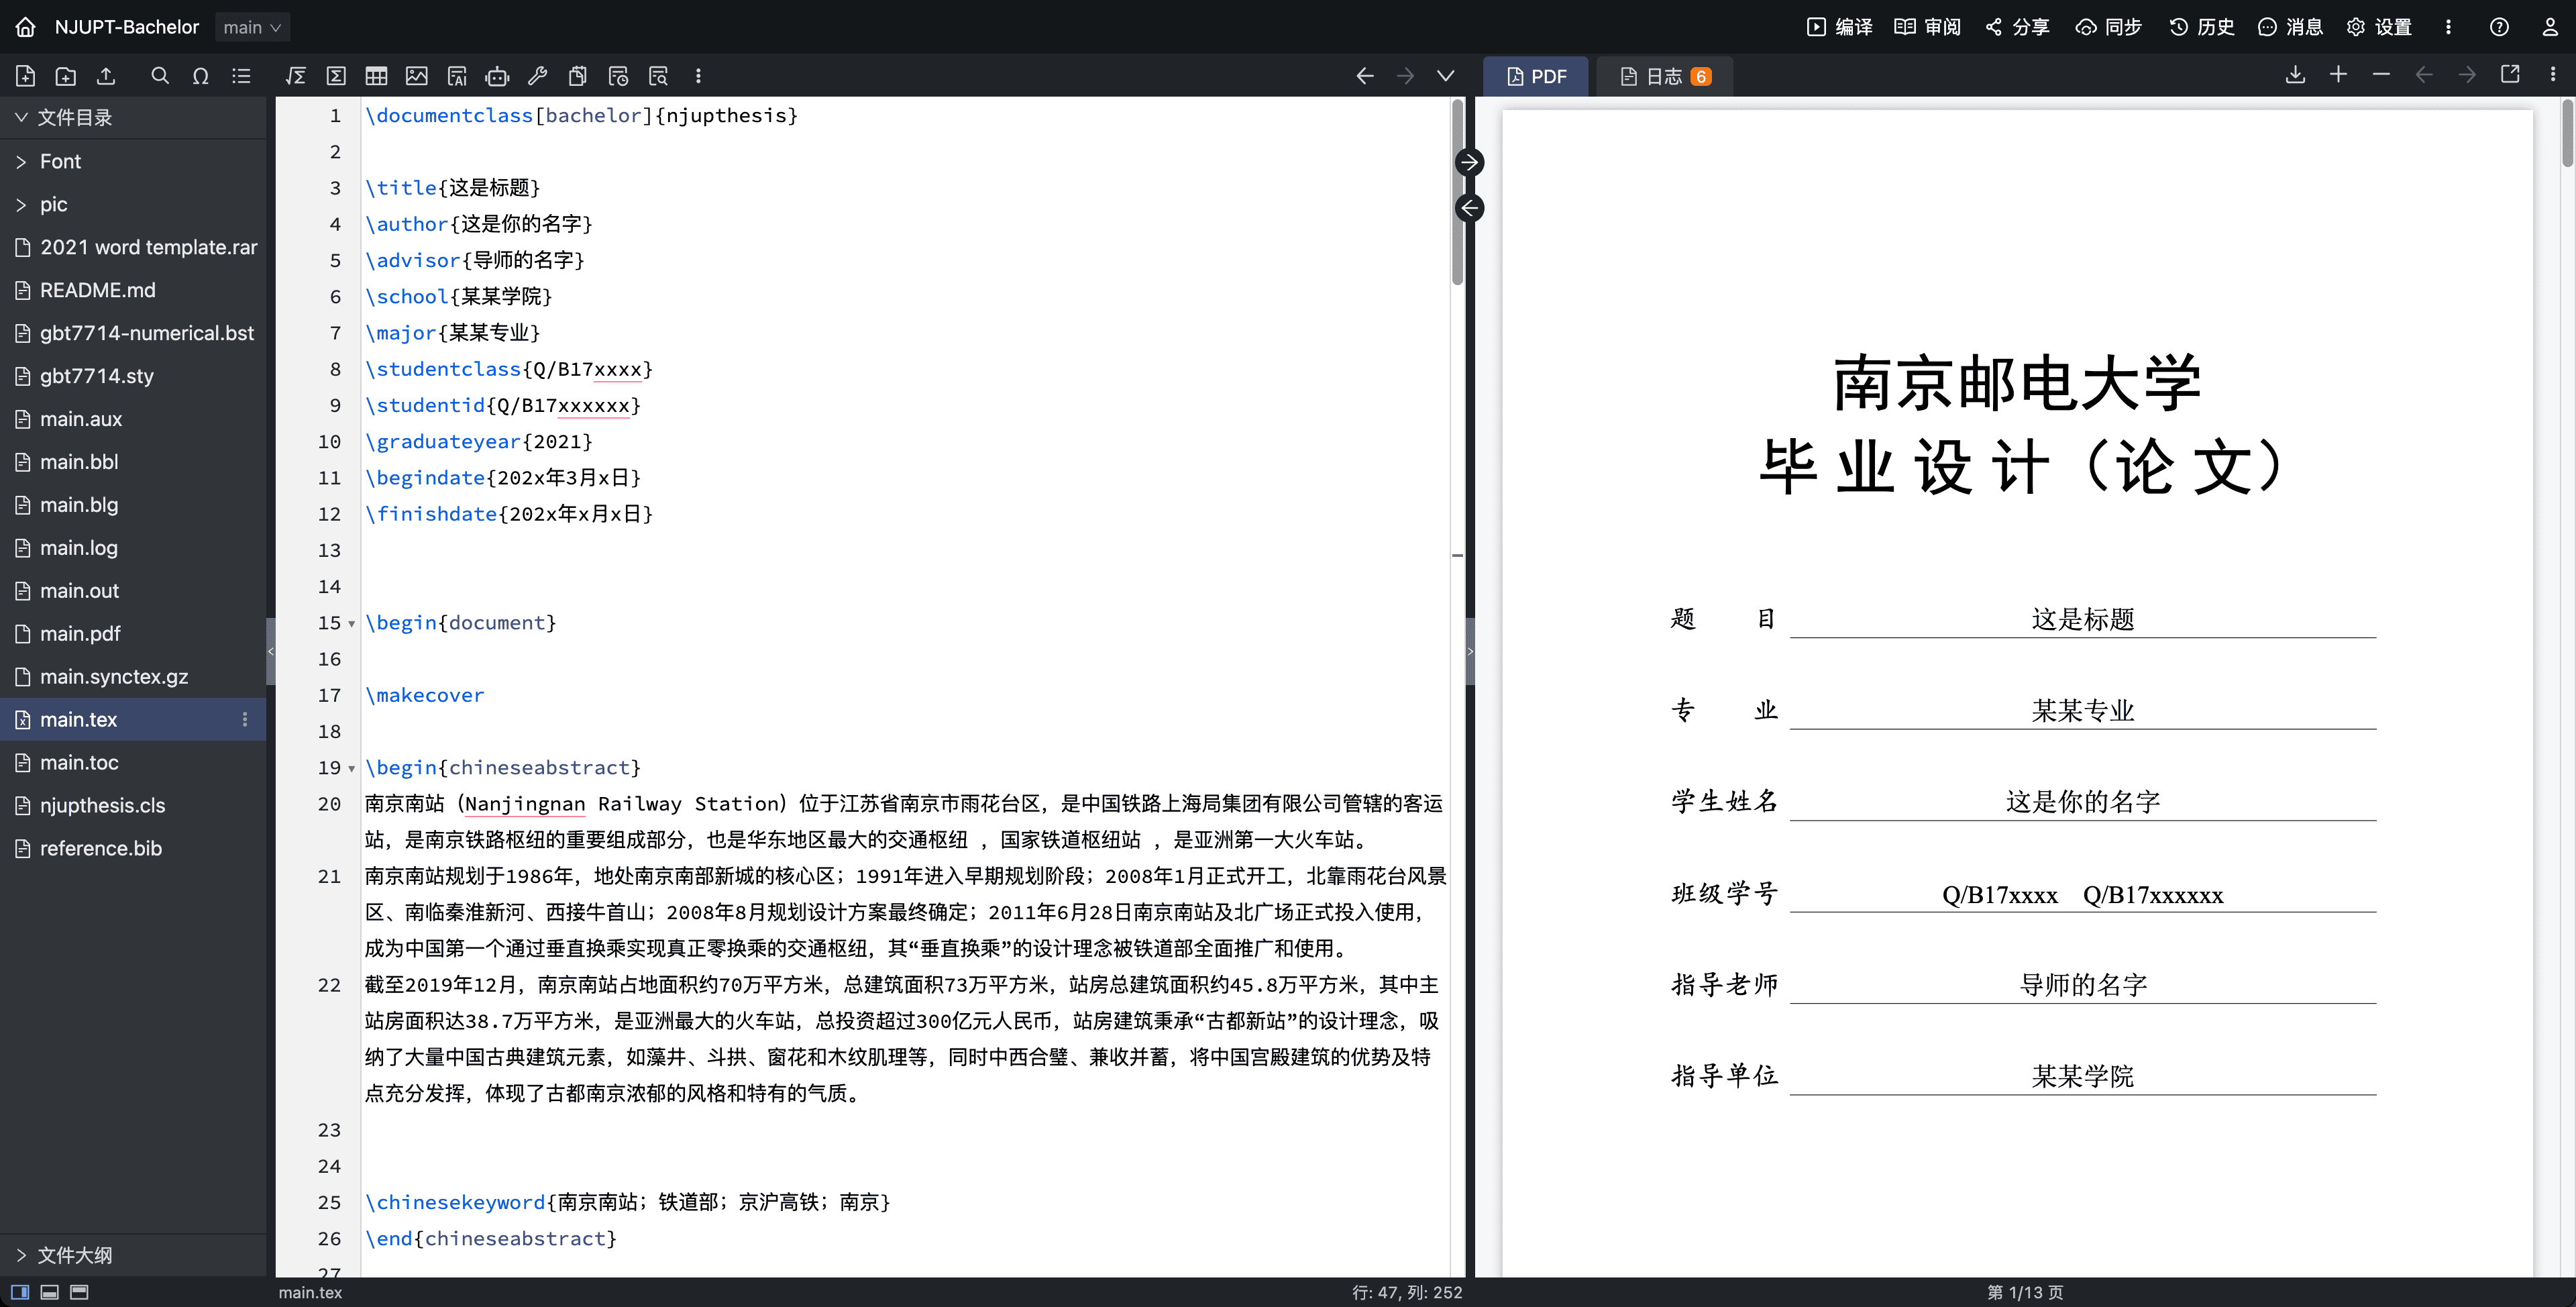
\includegraphics[width=0.8\textwidth]{texpage截图}
    \caption{这是一个texpage截图}
    \label{fig:2}
\end{figure}

图片下方会自动空出一行间距。

\newpage % 用这个符号可以直接换页,调整排版的时候能用得上

(3)多图片

下面演示多图片,每一个图片都可以单独设置width、label和图片的名字(在subfigure的第一个中括号里面)

我们可以直接引用其中的一个子图,南京南站如图\ref{南京南站:1}所示。

\begin{figure}[hbt]
	\centering
	\subfigure[南京南1]{
		\begin{minipage}[b]{0.4\textwidth}
			\includegraphics[width=1\textwidth]{1}
		\end{minipage}
	}
	\subfigure[南京南2]{
		\begin{minipage}[b]{0.4\textwidth}
			\includegraphics[width=1\textwidth]{2}
			
		\end{minipage}
	} \\
	\subfigure[南京南3]{
		\begin{minipage}[b]{0.4\textwidth}
			\includegraphics[width=1\textwidth]{3}
		\end{minipage}
	}
	\subfigure[南京南4]{
		\begin{minipage}[b]{0.4\textwidth}
			\includegraphics[width=1\textwidth]{4}
			
		\end{minipage}
		\label{南京南站:1}
	}
	\caption{南京南站}
	\label{南京南站}
\end{figure}

有的时候需要多张图片,但不需要给每一张图片命名,则使用下面的方式。这样生成出来的子图不会有abcd编号也不会有小图注。可以通过调整width里面的百分比来让俩图片大小一致。

\begin{figure}[hbt]
	\centering
	\subfigure{
		\begin{minipage}[b]{0.36\textwidth} % 调整百分比
			\includegraphics[width=1\textwidth]{1}
		\end{minipage}
	}
	\subfigure{
		\begin{minipage}[b]{0.4\textwidth}
			\includegraphics[width=1\textwidth]{2}
			
		\end{minipage}
	}
	\caption{南京南站}
	\label{南京南站1}
\end{figure}

(4)公式

这是一个公式,可以通过公式\ref{eq:1}指向这个公式。在latex中,所有label都可以通过ref来引用,包括图片、公式、表格。

\begin{equation}\label{eq:1}
	y=A x+b
\end{equation}

注意公式也需要是Times New Roman字体,如果用docx编辑必须要用mathtype插件才能实现新罗马字体(wps和word默认公式编辑都是改不了字体的),非常麻烦,这也是latex的优势。

(5)表格

下面给出表格的示例,注意学校的模板中表格是必须要与页面等宽的,latex默认的表格格式是不符合学校要求的。建议直接复制下面这个表格作为其他表格的模板。详情参考百分号\%之后的注释,使用表\ref{tab:1}引用这个表格。

\begin{table}[!htbp]
\centering
\caption{表格标题}
\label{tab:1}
\begin{tabularx}{\textwidth}{|Y|Y|c|} % 这里配置表格有几列,Y代表可伸缩列,c代表不可伸缩列,从结果来看可以看到最后一列是很窄的,因为不可伸缩。至少要保留一个Y列
    \hline
    第一列 & 第二列 & 第三列 \\
    \hline % 每一行之间的分割线,必须要有
    内容1 & 0 & 0 \\
    \hline
    内容2 & 0 & 0 \\
    \hline
\end{tabularx}
\end{table}

表格下方同样会有一个默认的空行。

\chapter{需要几章自己加一下!}

%这里是结束语
\thesisconclusion % 如果不需要结束语,删除这一行

结束语不一定需要编写,比如正文中最后一章是“总结与展望”则可以删除结束语部分。具体请咨询你的毕设指导老师,和老师确认是否需要结束语部分,以导师要求为准。

% 致谢区域
\thesisacknowledgement

本论文采用\LaTeX,基于南京邮电大学2025年理工艺教类的Word模板进行严格迁移编写。本模板开源地址:\url{https://github.com/musnows/NJUPT-Bachelor}。感谢 \href{https://github.com/dhiyu/NJUPT-Bachelor}{dhiyu}、\href{https://github.com/imguozr/NJUPThesis-Bachelor}{imguozr} 和 \href{https://github.com/lemoxiao/NJUPThesis-Scholar}{lemoxiao} 的工作,为本模板的形成奠定了坚实的基础。

% 参考文献区域
\thesisreference

%附录区域
\thesisappendix

注意:一般情况下不建议正文中出现无序列表或者有序列表,直接在正文中使用(1)和1.这两种方式编写即可。不确定学校是否接受论文中出现无序列表、有序列表、代码块。

\section{本科期间的学术成果发表情况}
\begin{itemize} % 无序列表
	\item 发表一篇Nature
	\item 获得了诺贝尔奖
	\item 当选足球先生
	\item 开发了1nm光刻机一台
\end{itemize}

\section{本科期间的获奖情况}
\begin{enumerate} % 有序列表
	\item 设计了一块RTX5090
	\item 准备移民火星
	\item 去太阳上面看看
\end{enumerate}

以下是一个代码块示例:

\lstset{language=bash} % 设置代码语言
\begin{lstlisting}[caption={更新Ubuntu软件}, label={code:apt-update}]
sudo apt-get update -y
sudo apt-get upgrade -y
\end{lstlisting}

\end{document} % 禁止删除,这是整个latex的结尾
